\documentclass[11pt, oneside]{article}   	% use "amsart" instead of "article" for AMSLaTeX format
\usepackage{geometry}                		% See geometry.pdf to learn the layout options. There are lots.
\geometry{letterpaper}                   		% ... or a4paper or a5paper or ... 
%\geometry{landscape}                		% Activate for rotated page geometry
%\usepackage[parfill]{parskip}    		% Activate to begin paragraphs with an empty line rather than an indent
\usepackage{graphicx}				% Use pdf, png, jpg, or eps§ with pdflatex; use eps in DVI mode
								% TeX will automatically convert eps --> pdf in pdflatex		
\usepackage{amssymb}

\usepackage{amsmath}

\DeclareMathOperator*{\argmax}{arg\,max}
\DeclareMathOperator*{\argmin}{arg\,min}
%SetFonts

%SetFonts


\title{Agent-based Reinforcement Learning in Colonel Blotto}
\author{Joseph Christian G. Noel}
\date{}							% Activate to display a given date or no date

\begin{document}
\maketitle

\section{Introduction}

In this paper we compare a reinforcement learning agent against a baseline random agent. It is shown that a reinforcement learning agent using the Q-Learning method handily beats basic baseline agents in Colonel Blotto.

\section{Colonel Blotto}


Colonel Blotto is a constant-sum game proposed by Émile Borel in 1921\cite{Borel1953}. In the game two or more players distribute resources (or coins) over several fronts in a battlefield. A player wins a front if they have allocated more resources to it than the other player. The objective of the game is to win more fields than your opponent.

\hfill

A notable thing about Colonel Blotto is that there is no optimal best strategy that will beat all other possible strategies. This means that the best strategy can change in a given game depending on the opponent and what the strategy the opponent is using. One way to play Colonel Blotto would be to update your strategy over time as you play the same opponent multiple times. If the opponent's strategy is constant or doesn't change much, it must be possible to eventually "learn" a strategy that would win against this opponent more often than it loses. In the field of 

\section{Reinforcement Learning}

Reinforcement Learning (RL) is a form of agent-based modeling. In RL an agent learns by performing actions which changes the state of an environment. After each action, the agent may also receive a "reward" whose value depends on how close the agent is to what it wants to achieve. The goal for the agent is to maximize the cumulative reward that it receives over all the actions that it takes. After a series of actions, the agent eventually reaches a goal state or terminal state, which signifies the end of an episode. The environment is then reset and the agent starts again from an initial state and the process then repeats itself.

\hfill

Formally, an RL model is a set of states $S$, a set of actions $A$, and transition rules between states depending on the action taken. For state $s \in S$ at time $t$, an agent performs an action $a \in A$, moves to a new state $s'$ and receives a reward $r_t$. The goal of the agent is to maximize the expected reward $Rt$,

\begin{equation}
R_t = \sum_{k=0}^{\infty}\lambda^kr_{t+k}
\end{equation}

where $0 \leq \gamma \leq 1$ is a discount factor for handling infinite horizons.

\hfill

$\pi(s,a)$ is a probability mapping of an agent taking action $a$ while in state $s$. A proper policy is one where there is a non-zero probability of reaching a terminal state. There is always an optimal policy $\pi^*$ that is better than or equal to all other policies when it comes maximizing the cumulative rewards. 

\subsection{Markov Decision Process}

A common formulation of the Reinforcement Learning problem is as a Markov Decision Process (MDP). In this class of RL problems, the information from the history of all states, actions, and rewards before time $t$ is encapsulate in the current state at time $t$. This is the Markov property, and tasks which exhibit this property are called Markov decision processes. Formally, the Markov property states that for transition probability function $Pr$,

\begin{equation}
Pr(s_{t+1}, r_{t+1} | s_t, a_t) = Pr(s_{t+1}, r_{t+1} | s_t,a_t, r_t, s_{t-1}, a_{t-1}, r_{t-1},...,s_0, a_0, r_0)
\end{equation}

\subsection{Value Function}
The state-action value function $Q$ is the estimate of the expected rewards the agent will receive by being at state $s$, at time $t$, taking action $a$, and then following policy $\pi$ from $t+1$ onwards. 

\begin{equation}
Q^\pi(s,a) = \mathbb{E}_\pi(R_t | s_t, a_t)
\end{equation}

The reinforcement learning problem can therefore be reduced to finding the optimal policy $\pi^*$ by simply choosing the action $a$ that maximizes $Q(s,a)$ for all $s \in S$ 

\begin{equation}
\pi^*(s) = \argmax_a{Q(s,a)}
\end{equation}
\subsection{Q-Learning}

Q-Learning is one of the basic reinforcement learning methods. It approximates the state-action value function $Q(s,a)$ using the Bellman equations, which allows it to define $Q(s,a)$ in a recursive manner. At each time step Q-Learning approximates the optimal policy in the following manner:

\begin{equation}
Q(s_t, a_t) = Q(s_t, a_t) + \alpha[r_{t+1} + \gamma \max_aQ(s_{t+1}, a_{t+1}) - Q(s_t, a_t)]
\end{equation}

where $\alpha > 0$ is the learning rate, and $0 \leq \gamma \leq 1$ is again the discount factor.

\section{Experiments}

We now show how how a Q-Learning agent performs against a random agent in Colonel Blotto.

\subsection{Experimental Setup}

We setup a 2-player Colonel Blotto game with 3 fields and 10 coins per player. This provides a total of 66 possible actions $a$ (ways to distribute the 10 coins on the 3 fields) that the players can choose from. The players aim to distribute their 10 coins among the 3 fields in such a way that their coins are greater than their opponent's coins in each field. The winner of the game is the player that wins more fields than their opponent, and received a reward of $r=1$ from the environment. The loser of the game receives a reward of $r=-1$. A single episode in reinforcement learning constitutes one game. We count how many games each player has won over time and show the results. .

\hfill

Our reinforcement learning agent uses the Q-Learning algorithm for approximating the optimal policy. We use $\alpha=0.1$ as the learning rate and $\gamma=1$ as the discount factor. We also set $\epsilon=0.2$ as the exploration rate for the agent. For the opponent, we use a RandomAgent that will select one of the 66 possible actions at random with equal probability for all of them. The experiments were run using the OpenSpiel\cite{OpenSpiel} environment simulator.


\subsection{Results}

We run 1000 games of Colonel Blotto to see the performance of the reinforcement learning agent. As shown in Figure 1, it takes almost 200 games before the RL agent really begins to start defeating the random agent regularly. In fact, if we look at the just the first 100 games (Figure 2), both agents win games at practically similar rates. However after 1000 games, the improved win rate of the RL agent can already be clearly seen.

\begin{figure}[h]
    \centering
    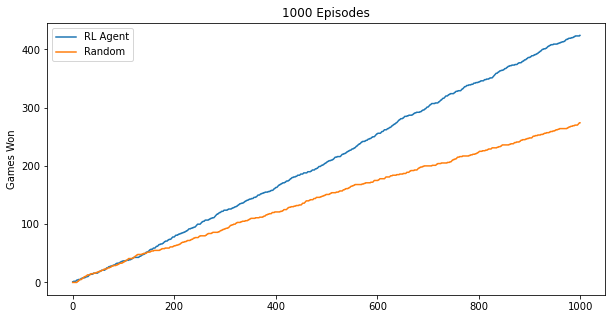
\includegraphics[scale=0.5]{./images/rl_random.png}
    \caption{Performance of RL Agent vs Random Agent}
    \label{fig:mesh1}
\end{figure}

\begin{figure}[h]
    \centering
    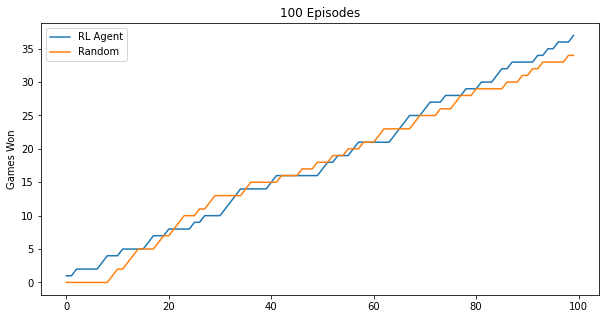
\includegraphics[scale=0.5]{./images/rl_random100.png}
    \caption{First 100 games of RL Agent vs Random Agent}
    \label{fig:mesh1}
\end{figure}

We also dive deeper and look at the $Q$-values that the agent has assigned to each of the 66 possible actions, to better understand what strategy it has arrived at. We also continue running the episodes to 1 million games to optimize the $Q$-values further before showing the results. Below we show the top 5 and the bottom 5 actions based on their $Q$-value scores. The 3 numbers for each action signify the number of coins that the RL agent assigns for each of the 3 fields.

\hfill

\begin{center}
\begin{tabular}{ |c| } 
 \hline
 \textbf{Top 4 Actions} \\ 
 \hline
 [4, 0, 6] \\ 
 \hline
 [5, 0, 5] \\ 
 \hline
 [0, 4, 6] \\
 \hline
 [6, 1, 3] \\

 \hline
\end{tabular}
\quad
\begin{tabular}{ |c| } 
 \hline
\textbf{Bottom 4 Actions} \\ 
 \hline
 [0, 0, 10] \\ 
 \hline
[0, 8, 2] \\
 \hline
 [0, 10, 0] \\
 \hline
 [10, 0, 0] \\
 \hline
\end{tabular}
\end{center}

As can be seen, the actions with the lowest $Q$-value are the ones where the agent puts all their coins in just one front, guaranteeing a loss when their opponent easily wins the other two fronts. On the opposite end, the best actions are the ones where the agent splits their coins almost evenly among just two fronts, with 0 coins allocated to the third front. By sacrificing one of the fronts, they give themselves the best chance to win the other two fronts they focused on, and have a high probability of winning the game in the process. Against a Random Agent, this results in the high win rates that were shown in the earlier graphs.

\section{Conclusion}

We have shown how a RL agent using Q-Learning performs against a Random Agent in 1000 games of Colonel Blotto. The RL doesn't do at well at first, and actually has quite similar win rates to the Random Agent over the first 100 to 150 episodes. It takes almost 200 episodes for the RL agent to start differentiating itself to the Random Agent, and by 1000 episodes the RL agent has started to clearly show its dominance.

\hfill

We also investigated what strategies the RL agent has learned through its repeated playing, and find that its preferred strategy is to sacrifice one of the fronts and focus on the other 2 fronts, splitting its coins almost evenly between them. This was shown empirically to be a a winning strategy against the Random Agent

\nocite{*}
\bibliographystyle{abbrv}
\bibliography{References}


\end{document}  